\section{Functions and Continuity} 

  Note that from set theory, we can construct functions as a subset of Cartesian product of two spaces $X, Y$. There is nothing new here. 

  \begin{definition}[Continuous Function]
    A function $f$ between 2 topological spaces $(X, \T_{X})$ and $(Y, \T_{Y})$ is \textbf{continuous at $x \in X$} if the preimage of every open neighborhood of $f(x) \in Y$ is an open neighborhood of $x \in X$.
    \begin{equation}
      U_{f(x)} \in \T_{Y} \implies x \in f^{-1}(U_{f(x)}) \in \T_{X}
    \end{equation} 
    $f$ is said to be \textbf{continuous} (at all points) if the preimage of every open set in $Y$ is an open set in $X$.\footnote{Note that continuity of a function $f$ is not only determined by the function itself, but also by the topologies of $X$ and $Y$.}
  \end{definition}

  Note that it is easier for $f$ to be continuous when the $\T_X$ is finer (since there are more open sets in $X$ for the preimage of $V \subset Y$ to map to) or $\T_Y$ is coarser (since there are fewer open sets that we have to check to map to open sets of $X$). 

  \begin{theorem}[Sufficient Properties for Continuity]
    Let $X, Y$, be topological spaces and let $f: X \longrightarrow Y$. Then, the following are equivalent to $f$ being continuous. 
    \begin{enumerate}
      \item The preimage of every basis element $B \in \T_Y$ is open in $X$. 
      \item For every closed set $B$ in $Y$, the set $f^{-1} (B)$ is closed in $X$. 
      \item For every subset $A$ of $X$, $f(\bar{A}) \subset \bar{f(A)}$. 
    \end{enumerate}
  \end{theorem}  
  \begin{proof}
    Listed. 
    \begin{enumerate}
      \item An arbitrary open set $V$ of $Y$ can be written as $V = \cup_{\alpha \in J} b_\alpha$. Then, 
      \begin{equation}
        f^{-1} (V) = f^{-1} \Big( \bigcup_{\alpha \in J} b_\alpha \Big) = \bigcup_{\alpha \in J} f^{-1} (b_\alpha)
      \end{equation}
    \end{enumerate}
  \end{proof}

  Great, so we have a few ways in which we can check continuity of a function. There are a few special cases. 

  \begin{lemma}[Trivially Continuous Functions]
    We have the following for general topological spaces. 
    \begin{enumerate}
      \item The identity function $\id: (X, \T_1) \rightarrow (X, \T_2)$ is continuous if $\T_1 \supset \T_2$. 
      \item A constant function $f: (X, \T) \rightarrow (Y, \T_2)$ is always continuous, regardless of the topologies. 
    \end{enumerate}
  \end{lemma}
  \begin{proof}
    If we take an open set $U \in \T_2$, its preimage is the same set $U$, which is guaranteed to be in $\T_1$ since $\T_1$ is finer than $\T_2$. 
  \end{proof}

  \begin{lemma}[Composition of Continuous Functions]
    If $f: X \rightarrow Y$ and $g: Y \rightarrow Z$ is continuous, then $g \circ f :X \rightarrow Z$ is continuous. 
  \end{lemma}

\subsection{Construction of Continuous Functions} 

  \begin{theorem}[Arithmetic on Real Continuous Functions]
    If $X$ is a topological space, and if $f, g: X \longrightarrow \mathbb{R}$ are continuous, then $f + g$, $f-g$, and $f \cdot g$ are also continuous. $f / g$ is continuous if $g(x) \neq 0$ for all $x \in X$. 
  \end{theorem}

  \begin{theorem}[Analytic Continuity = Topological Continuity] 
    Given metric spaces with their induced metric topologies $(X, \T_X, d_X)$ and $(Y, \T_Y, d_Y)$. The following are equivalent. 
    \begin{enumerate}
      \item $f: X \rightarrow Y$ is continuous at $x$. 
      \item For every $\delta > 0$, there exists an $\epsilon = \epsilon(\delta) > 0$ such that for all $z \in X$, $d_X (x, z) < \epsilon \implies d_Y (f(x), f(x)) < \delta$.\footnote{This is the definition of continuity at a point in analysis.} 
    \end{enumerate}
  \end{theorem}
  \begin{proof}
    ($\rightarrow$) Assume $f$ is continuous according to the $\epsilon - \delta$ definition. Let $U$ be any open set in $Y$ containing the point $y$, and let $x$ be an element in $f^{-1}(U)$ such that $y = f(x)$. We must prove that $f^{-1}(U)$ is also open. Since open sets contain neighborhoods (e.g. open balls) of all of its points, we can claim that, since $U$ is open by assumption, there exists an open ball $B_y$ around $y$ with radius $\epsilon > 0$. This guarantees the existence of a point $z \in U$ such that $\rho(y, z) < \epsilon$ for any $\epsilon > 0$ that we choose. Since $f$ is continuous, for every $\epsilon >0$ that we chose previously, there exists a $\delta >0$ such that $d(x, w) \implies \rho(f(x), f(w)) < \epsilon$. Since $\rho(f(x), f(w)) < \epsilon$, we can conclude that $f(w) \in B_y \subset U$ when $d(x, w) < \delta$. Therefore, $d(x, w) < \delta \implies w \in f^{-1}(U)$. But this is equivalent to saying that if $w \in B_(x, \delta)$, then $w \in f^{-1}(U)$, which means that every single point $x \in f^{-1}(U)$ contains an open ball neighborhood fully contained in $f^{-1}(U)$. So, by definition, $f^{-1}(U)$ is open. 


    ($\leftarrow$) Assume $f^{-1}(U)$ is open when $U$ is an open set in $Y$, i.e. $f$ is continuous under the topological definition. Let us define the open ball 
    \[ B(f(x), \epsilon) \equiv \{ y \in Y \; | \; \rho(f(x), y) < \epsilon\} \in \tau_Y\]
    By our assumption, $f^{-1} \big( B(f(x), \epsilon) \big)$ is an open set in $\tau_X$, and clearly, $x \in f^{-1} \big( B(f(x), \epsilon) \big)$ since $f^{-1}$ maps the point $f(x) \in B(f(x), \epsilon)$ to $x \in f^{-1} \big( B(f(x), \epsilon) \big)$. But since $f^{-1} \big( B(f(x), \epsilon) \big)$ is open, we can construct an open ball around $x$ with radius $\delta$ fully contained within the open set. Moreover, by selecting a point $p \in B(f(x), \delta) \subset f^{-1}\big( B(f(x), \epsilon) \big)$, we can guarantee that $f(p) \in B(f(x), \epsilon)$. This is precisely the $\epsilon - \delta$ definition of continuity. That is, given an $\epsilon > 0$ to be the radius of an open ball $B(f(x), \epsilon)$ in $Y$, we can always choose a $\delta > 0$ to be the radius of the open ball $B(x, \delta)$ in $X$ that is fully contained within the preimage of $B(f(x), \epsilon)$. In mathematical notation, 
    \[ p \in B(x, \delta) \subset f^{-1} \big( B(f(x), \epsilon) \big) \implies f(p) \in f\big( B(x, \delta) \big) \subset B(f(x), \epsilon)\]
    or equivalently in terms of metrics,
    \[ d(x, p) < \delta \implies \rho (f(x), f(p)) < \epsilon\]
  \end{proof} 

\subsection{Sequences}

  \begin{definition}[Sequence]
    A sequence $(x_\alpha)$ of points in topological space $(X, \T)$ is said to \textbf{converge} to the point $x \in X$ if for every neighborhood $U$ of $x$ there exists a $N \in \mathbb{N}$ such that
    \begin{equation}
      x_n \in U \text{ for all } n \geq N
    \end{equation}
  \end{definition}

\subsection{Homeomorphisms}

  \begin{definition}[Homeomorphism]
    A bijective, bicontinuous function $f: X \longrightarrow Y$ between two topological spaces is called a \textbf{homeomorphism} between $X$ and $Y$. If there exists at least one homeomorphism between $X$ and $Y$, then $X$ is said to be \textbf{homeomorphic} to $Y$, denoted $X \cong Y$. 

    \begin{figure}[H]
      \centering 
      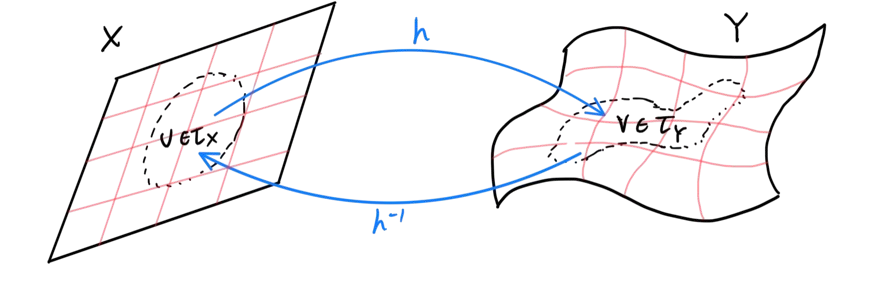
\includegraphics[scale=0.4]{img/Homeomorphism_of_Plane.png}
      \caption{The visual below shows a homeomorphism between the plane $X$ and the surface $Y$.}
      \label{fig:homeomorphism_plane}
    \end{figure}
  \end{definition}

  \begin{theorem}[Sufficient Properties of Homeomorphism]
    Suppose $f: X \rightarrow Y$ is a bijection. TFAE. 
    \begin{enumerate}
      \item $U \subset Y$ is open iff $f^{-1} (U)$ is open. 
      \item $U \subset X$ is open iff $f(U)$ is open. 
      \item $f$ is a homeomorphism. 
    \end{enumerate}
  \end{theorem} 

  Note that we may have functions that are bijective and continuous, but not bicontinuous. In order to construct such examples one of the easiest things we can do is just endow the codomain with the discrete topology, which guarantees continuity. 

  \begin{example}[Bijective and Continuous but not Homeomorphism]
    $\mathbb{Z}$ and $\mathbb{Q}$ are countable sets, so there is a bijection between them. If we give each of them the metric topology, $\mathbb{Z}$ ends up having the discrete topology (take the $0.5$-ball around each integer), whereas for $\mathbb{Q}$, we will see later that by the density of the rationals there are an infinite number of rationals in $(q - r, q + r)$ for $q \in \mathbb{Q}$. Note that this bijection $f: \mathbb{Z} \rightarrow \mathbb{Q}$ is continuous (since $\mathbb{Z}$ has discrete topology) but not bicontinuous. 
  \end{example}


  \begin{example}[Comparability and Homeomorphic Spaces]
    Consider the set $X = \{a, b\}$ with the two topologies $\T_3 = \{\emptyset, \{a\}, X\}$ and $\T_4 = \{\emptyset, \{b\}, X\}$. They are not comparable but they seem ``similar'' in a way in that if we swap all the $a$'s and $b$'s in $\T_3$, then we get $\T_4$. We can make this rigorous by defining $f: (X, \T_3) \rightarrow (X, \T_4)$ with $f(a) = b, f(b) = a$, and showing that it is a homeomorphism. 
  \end{example}

  In fact, a homeomorphism $f$ is an equivalence relation between two topological spaces. This partitions the set of all topological spaces into \textbf{homeomorphism classes}. Analogous to how isomorphisms preserve algebraic structures, homeomorphisms preserve topological structure between topological spaces. 

  \begin{example}[Homeomorphism Classes of 2D Manifolds]
    There is an infinite family of 2-dimensional manifolds, call them $M$ and $N$, and each set in each family is not homeomorphic to another.  
    \begin{enumerate}
      \item $M_0 = S^2$ (sphere). $M_1 = T^2$ (torus). $M_2$ is a donut with two holes. $M_3$ has three holes, and so on. 
      \item $N_1$ is the Mobius strip. $N_2$ is the Klein bottle. 
    \end{enumerate}
  \end{example}

  Additionally, not only does a homeomorphism give a bijective correspondence between points in $X$ and $Y$, but it also determines a bijection between \textbf{the set of all open sets in $X$ and $Y$} (that is, a bijection between their topologies)! This bijection then allows two spaces that are homeormophic to have the same topological properties. 

  \begin{theorem}[Preservation of Topological Properties]
    A homeomorphism $f$ between two topological spaces $(X, \tau_{x})$ and $(Y, \tau_{Y})$ preserves all topological properties (e.g. separability, countability, compactness, (path) connectedness) of $X$ onto $Y$ and $Y$ onto $X$. 
  \end{theorem}

  \begin{definition}[Embedding]
    Suppose that $f: X \longrightarrow Y$ an injective continuous map with $X, Y$ topological spaces. Let $Z \equiv \im{f}$. Then, the function
    \begin{equation}
      f^\prime: X \longrightarrow Z \subset Y
    \end{equation}
    obtained by restricting the codomain of $f$ is bijective. If $f^\prime$ happens to be a homeomorphism of $X$ with $Z$, then we say that the map
    \begin{equation}
      f: X \longrightarrow Y
    \end{equation}
    is a \textbf{topological embedding}, or more simply an \textbf{embedding}, of $X$ in $Y$. 
  \end{definition} 

  A homeomorphism can be useful, but we can work a lot more flexibly with it by knowing that the restriction of a homeomorphism is a homeomorphism. 

  \begin{theorem}[Restriction of Homeomorphism is Homeomorphism]
    If $f: X \rightarrow Y$ is a homeomorphism, then for any $x \in X$, the restriction 
    \begin{equation}
      f|_{X \setminus \{x\}} : X \setminus \{x\} \rightarrow Y \setminus \{f(x)\}
    \end{equation}
    is also a homeomorphism. 
  \end{theorem}

\subsection{Hausdorff Axiom (To be Moved)} 

  \begin{lemma} 
    For any metric space, the metric topology is Hausdorff. 
  \end{lemma}

  \begin{lemma} 
    $X$ Hausdorff implies any sequences converges to at most one point. 
  \end{lemma}

  \begin{lemma} 
    $X$ Hausdorff implies any finite subset is closed. 
  \end{lemma}

  \begin{example}
    $X$ is an infinite set, then finite complement topology is not Hausdorff. 
  \end{example} 

  \begin{definition}
    One point sets are closed is the $T_1$ axiom. Equivalently, for any pair $x_1 \neq x_2$, there is an open set $U$ s.t. $x_1 \in U$ and $x_2 \not\in U$. 
  \end{definition}

  \begin{example}[Line with Two Origins]
    $X = \mathbb{R} \setminus \{0\} \cup \{0_1, 0_2\}$ with basis given by intervals $(a, b)$ for $b < 0$ or $a > 0$, and $(a, 0) \cup \{0_i\} \cup (0, b)$ for $a < 0 < b$. 
  \end{example}

